% vim: set tw=78 sts=2 sw=2 ts=8 aw et ai:

Having been on the market for 6 years, the Android operating system and the
environment around it have evolved continuously in reply to user demand. With
this growth in popularity the need for providing adequate security for
personal data has been increasingly pronounced.

While safety mechanisms have always been present in Android, it was only
recently\cite{android-layers} that the Android Security Team highlighted the
protection features available on more than half of the smartphones sold
globally. A summary can be seen in Figure \ref{fig:layers}. With so many
checks and analysis being done both on Google servers and on the device
itself, successfully compromising a smartphone is increasingly difficult for
an attacker and consequently innovative manners of bypassing these filters
have been developed.

\begin{figure}[hb]
  \centering
  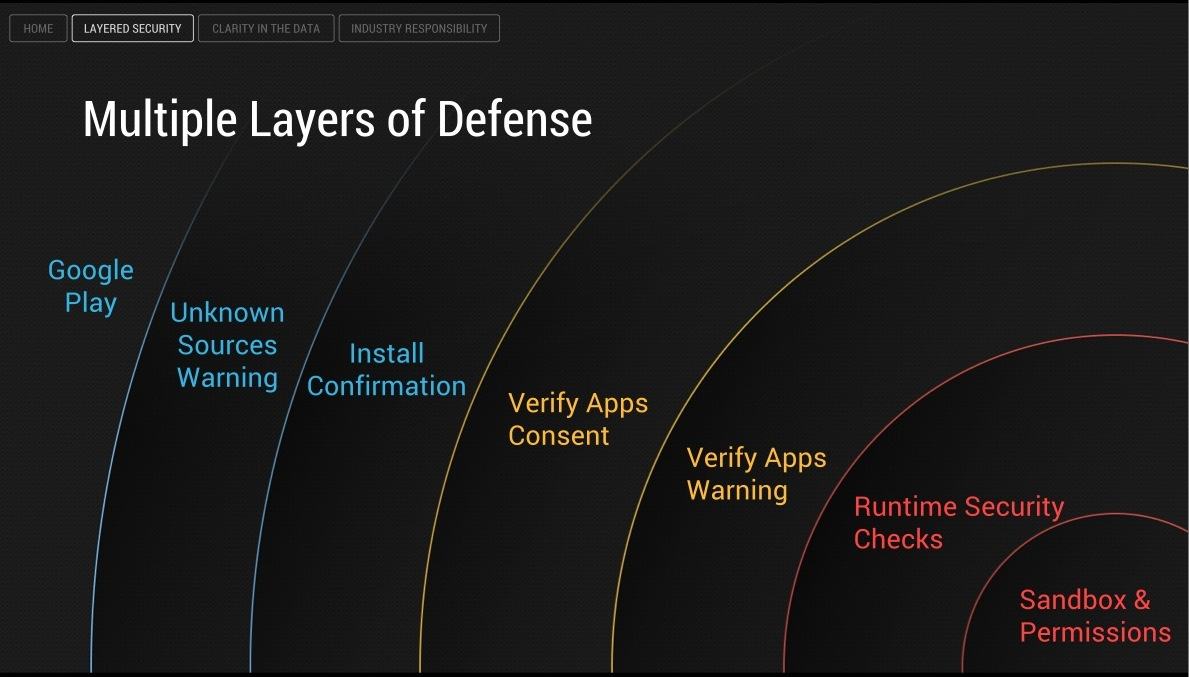
\includegraphics[width=0.5\textwidth]{img/android-layers}
  \caption{Android Security Layers - Image courtesy of Andrian Ludwig}
  \label{fig:layers}
\end{figure}

One approach employed by malicious agents is to use picture files bundled with
the Android application. Normally pictures are bundled with applications for
cosmetic purposes and therefore ignored and considered harmless. However,
there is nothing preventing a determined attacker to use such a file as a
wrapper for hiding a harmful payload. Basically, the original application is a
trojan, indistinguishable from an ordinary application.

The first incident of this type has been reported in September
2011\cite{droid-coupon}. An application called DroidCoupon pretended to offer
various coupons in order to lure users to download it. However, it used an
image file to hide a local privilege exploit. For all intents and purposes the
special file behaved like an image file, but the DroidCoupon application,
reading from a custom offset, extracted the local exploit and used it to gain
root access on the smartphone. From that point, the attacker could violate
security protections and leak private user data.

As time progressed, so has the complexity of the techniques used by attackers.
In 2013, the Gamex malware also used an image file to hide the malicious
payload\cite{hiding-apk}. However, its approach was a little more elegant. A
file with the PNG extension was, in fact, a ZIP archive and by default would
extract harmless files. Nevertheless, if the ZIP archive was XOR-ed with a
certain key it produced another valid ZIP, which contained the malicious
payload. This was a significand step up from previous incidents, as
recognizing such behavior was not a trivial task.

Last but not least, in 2014, researchers went a step further\cite{hiding-apk}.
Although the behavior of Gamex was atypical, the fact that it used XOR
encryption meant that subsequent tentatives of the same manner could be
thwarted. Therefore, they employed the cryptographic ciphers exposed by the
Android framework in a rather unorthodox manner. In addition, they relied on
the fact that parsers for specific file formats are error-prone. As a result,
they managed to encrypt a PNG file using AES in CBC mode and obtain a valid
APK file, an Android application that could be installed on the victim
software. Using a standardized encryption algorithm to hide the malicious
payload renders any analysis useless as it is computationally infeasible to
crack AES.

Having outlined previous work with regards to the problem we attempt to solve,
we will now take into account prior research that may aid in the development
of an effective countermeasure. Since the current trend seems to be using more
secure cryptographic ciphers, namely the ones provided by the Android
framework itself, we consider instrumenting the framework itself a valid
approach. More to the point, we wrap methods from Android's cryptographic API
and look for valid file headers in both the input and the output. Normally,
depending whether we are encrypting of decrypting, either the input or the
output should have a valid file signature, while the other should seem random.
If both are not random, then there is a high probability that we are
witnessing a tentative attack.

There are a few instrumentation frameworks available for the Android platform.
Most are geared towards modifyig the user interface and adding features. They
provide complex functionality. Therefore, they are not trivial to setup and,
considering out target are cryptographic operations, may add non-negligible
overhead.

Thankfully, security researchers have developed simplified
alternatives. While lacking in features when compared with more
mature instrumentation frameworks, DDI\cite{ddi} is lightweight and will not
induce a high computational overhead. It works by injecting a library in the
Dalvik runtime that replaces the original entry points to the methods of
interest. The Dalvik virtual machine is the part of the Android operating
system that runs the individual applications. Therefore, a wrapper function
here can be applied to the method of our choice in the context of the
application we wish to monitor.
